% Narrative source. build_report.py generates the pinned tables and figures only.
\documentclass[10pt,a4paper]{article}
\usepackage{fontspec}
\setmainfont{texgyretermes}[Extension=.otf,UprightFont=*-regular,BoldFont=*-bold,ItalicFont=*-italic,BoldItalicFont=*-bolditalic]
\usepackage[margin=1.8cm,headheight=14pt]{geometry}
\usepackage{amsmath,amssymb,booktabs,tabularx,array,ragged2e,enumitem,microtype,xcolor,tikz,fancyhdr,graphicx,titlesec}
\usetikzlibrary{arrows.meta,positioning}
\usepackage[hidelinks,unicode]{hyperref}
\definecolor{ink}{HTML}{183A45}
\definecolor{teal}{HTML}{087F7A}
\definecolor{blue}{HTML}{405F8A}
\definecolor{gray}{HTML}{56656B}
\definecolor{orange}{HTML}{976440}
\newcolumntype{P}[1]{>{\RaggedRight\arraybackslash}p{#1}}
\newcolumntype{Y}{>{\RaggedRight\arraybackslash}X}
\setlength{\parindent}{0pt}\setlength{\parskip}{5pt}\setlength{\emergencystretch}{2em}
\setlength{\tabcolsep}{4pt}\renewcommand{\arraystretch}{1.16}
\setlist{nosep,leftmargin=1.4em,topsep=3pt}
\titleformat{\section}{\large\bfseries\color{ink}}{\thesection}{.6em}{}
\titleformat{\subsection}{\normalsize\bfseries\color{ink}}{\thesubsection}{.6em}{}
\titlespacing*{\section}{0pt}{8pt}{6pt}
\titlespacing*{\subsection}{0pt}{7pt}{4pt}
\pagestyle{fancy}\fancyhf{}
\fancyhead[L]{\small\color{gray}BẢO VỆ RIÊNG TƯ BẰNG GEO-I / REM}
\fancyhead[R]{\small\color{gray}Cơ chế và bằng chứng}
\fancyfoot[C]{\small\thepage}\renewcommand{\headrulewidth}{0.3pt}
\newcommand{\key}[1]{\par\smallskip\noindent\textcolor{teal}{\textbf{#1}}\par\smallskip}
\hypersetup{pdftitle={Bảo vệ riêng tư truy vấn và quỹ đạo bằng Geo-I/REM},pdfauthor={}}
\newcommand{\UtilityRows}{Gần nhất & 92,45 & 94,68 & +2,23\\
Nhanh nhất & 92,45 & 94,68 & +2,23\\
Trong bán kính & 81,69 & 86,88 & +5,18\\
Ít vòng đường nhất & 92,27 & 94,52 & +2,25\\
Trung bình đều bốn mục đích & 89,71 & 92,69 & +2,97\\}
\newcommand{\PrivacyRows}{S4: cùng người & AUC $\downarrow$ & 0,778 & 0,532 & Geo-I lịch sử\\
S4: cùng xe & AUC $\downarrow$ & 0,718 & 0,448 & Geo-I lịch sử\\
S5 & Đúng cạnh $\downarrow$ (\%) & 100,00 & 50,00 & Epoch8 / L20\\
S6 & Hit100 $\downarrow$ (\%) & 100,00 & 50,00 & Epoch8 / L20\\
S9 & MAE $\uparrow$ (m) & 790 & 1407 & Endpoint20 riêng\\
S10 & MAE $\uparrow$ (m) & 758 & 1337 & Endpoint20 riêng\\}
\newcommand{\TimelineRows}{0 & Có & Tạo mới & Cập nhật & 1u & 1/23\\
20 & Không & Giữ & Dự đoán & 0u & 1/23\\
60 & Có & Tạo mới & Cập nhật & 2u & 3/23\\
120 & Có & Tạo mới & Cập nhật & 2u & 5/23\\
600 & Có & Tạo mới & Cập nhật & 2u & 21/23\\}

\begin{document}
\begin{center}
{\LARGE\bfseries\color{ink}Bảo vệ riêng tư truy vấn và quỹ đạo}\\[3pt]
{\large Geo-I / REM, mạng đường và xử lý nhu cầu tại thiết bị}
\end{center}

\section{Cơ chế bảo vệ nội dung và các scenario còn lại}
\textbf{Nền tảng giữ nguyên:} GPS được bảo vệ bằng Geo-I/REM để tạo hoặc giữ tham chiếu $Z$.
Thiết bị ước lượng phân bố $b$ từ lịch sử đã bảo vệ, rồi chọn $K=5$ tọa độ truy vấn $Q$ khả thi theo mạng đường.
Máy chủ thấy $Q$ và lịch gửi, không nhận GPS thật, $Z$, nhu cầu $\psi$ hoặc đáp án local.

\subsection{S7: giữ nhu cầu thật local, truy hồi một tập ứng viên chung}
Nhu cầu thật $\psi$ gồm loại POI, tiêu chí, bán kính hoặc đích riêng. Máy chủ luôn nhận cùng yêu cầu:
mọi loại POI công khai, độ sâu cố định $L=30$ tại mỗi $Q$. Sau khi nhận phản hồi, thiết bị mới gộp,
bỏ trùng ID và dùng GPS cùng $\psi$ để lọc, sắp xếp danh sách phù hợp.
\[
5Q\times L30\ \longrightarrow\ \leq150\text{ bản ghi mỗi loại}
\ \longrightarrow\ \text{nhận, bỏ trùng}\ \longrightarrow\ \text{lọc và sắp xếp local}.
\]
Con số 150 là trần trước bỏ trùng, không phải 150 POI duy nhất hay trần cho toàn bộ sáu loại POI.
Truy hồi mọi loại đã có từ trước; phần mở rộng là bốn nhu cầu local và kiểm tra yêu cầu mạng bất biến khi đổi nhu cầu.

\par\smallskip
\begin{tabularx}{\linewidth}{@{}P{3.4cm}Y@{}}\toprule
\textbf{Nhu cầu local} & \textbf{Tiêu chí lọc / sắp xếp}\\\midrule
Gần nhất & Khoảng cách đường $D_G(x,p)$.\\
Đến nhanh nhất & Thời gian đường thông thoáng $T_G(x,p)$; chưa gồm ùn tắc.\\
Trong bán kính $r$ & Giữ $D_G(x,p)\leq r$, rồi sắp theo khoảng cách.\\
Ít đi vòng tới đích $a$ & $D_G(x,p)+D_G(p,a)-D_G(x,a)$; đích $a$ chỉ dùng local.\\\bottomrule
\end{tabularx}

\key{S7: cùng trạng thái đã bảo vệ và lịch công khai, đổi nhu cầu $\psi$ không đổi $Q$, payload, lịch hoặc số request.}
Độ gần là cách thu ứng viên cho dịch vụ lân cận, không bắt mọi nhu cầu chọn POI gần nhất.
Đủ đáp án chỉ khi pool chứa các POI cần thiết. Số POI hiển thị không quyết định cơ chế S7;
triển khai và benchmark vẫn dùng $k=5$, Recall@5. Tương quan ý định--tuyến đường và click còn là kênh suy luận.

\subsection{S4, S5, S6: hỗ trợ gián tiếp, chưa có bảo vệ chuyên biệt đầy đủ}
\par\smallskip
\begin{tabularx}{\linewidth}{@{}P{.8cm}P{3.25cm}Y@{}}\toprule
\textbf{Case} & \textbf{Attacker muốn biết} & \textbf{Cơ chế và khó khăn}\\\midrule
S4 & Cùng người hoặc cùng xe qua phiên & Cap chung giới hạn tọa độ tích lũy. Account/IP, hình dạng và thói quen vẫn có thể liên kết danh tính.\\
S5 & Cạnh đường sắp đi & Geo-I, lịch đọc và cap làm mờ prefix. $Q$ không dùng tương lai thật; hình học vẫn có thể tiết lộ hướng rẽ.\\
S6 & Đích chưa tới & Bảo vệ tọa độ trong lịch sử và prefix; đích riêng không gửi theo query. Routine qua nhiều chuyến vẫn có thể gợi ý đích.\\\bottomrule
\end{tabularx}

$b$ và bộ chọn $Q$ phục vụ utility, không phải bộ chống dự đoán độc lập. Pilot S5/S6 mới xét hai ứng viên.
\textbf{S8} là suy vị trí qua người đồng hành: đã có diagnostic lịch sử, chưa xác nhận cơ chế cấp nhóm.
Giữ S8 như giới hạn phạm vi, không dành phần trình bày riêng hoặc tuyên bố đã giải quyết S1--S10.
{\small\color{gray}Nền nghiên cứu: Geo-I (Andrés, 2013), predictive composition (Chatzikokolakis, 2014);
nhận dạng quỹ đạo (de Montjoye, 2013), dự báo hành trình (Ziebart, 2008), interdependent privacy (Olteanu, 2017).}

\clearpage
\section{Cap tám phiên và lập luận riêng tư}
\textbf{Vì sao thêm cap liên phiên?} Geo-I giới hạn thông tin mỗi lần đọc được bảo vệ, nhưng nhiều lần quan sát vẫn hợp thành.
Nếu mỗi chuyến tự được cấp lại toàn bộ ngân sách, attacker có thể gom các chuyến để tăng thông tin về vị trí và routine.
Sổ chung bổ sung giới hạn tích lũy cho Geo-I, hỗ trợ S2/S3 và phần tọa độ của S4.

\textbf{Phiên} là một chuyến; \textbf{epoch} là nhóm tối đa $N=8$ phiên được cấp theo chính sách công khai.
Sổ lưu bền vững qua khởi động lại; dành slot trước GPS và không hoàn phần dư dựa trên nhánh bí mật.
\par\smallskip
\begin{tabularx}{\linewidth}{@{}P{4.5cm}Y Y@{}}\toprule
\textbf{Phân bổ} & \textbf{Bản trước} & \textbf{Epoch8 hiện tại}\\\midrule
Cap mỗi phiên & $0{,}23/\mathrm m$ & $0{,}02875/\mathrm m$\\
Tổng cận tám phiên & $1{,}84/\mathrm m$ nếu cấp lại từng chuyến & $0{,}23/\mathrm m$ dùng chung\\
Đơn vị phí $u$ & $0{,}01/\mathrm m$ & $0{,}00125/\mathrm m$\\\bottomrule
\end{tabularx}
\[
C_{\rm epoch}=0{,}23/\mathrm m,\qquad C_{\rm phiên}=C_{\rm epoch}/8=0{,}02875/\mathrm m,
\]
\[
H=12,\qquad U=2H-1=23,\qquad u=C_{\rm phiên}/U=0{,}00125/\mathrm m.
\]
$U$ là số đơn vị phí của một phiên. $H=12$ không buộc đúng 12 lần GPS; tám phiên cũng không phải tám lần đọc.
Ngân sách danh nghĩa phiên $0{,}03/\mathrm m$ khác cap hiệu lực $0{,}02875/\mathrm m$.

\subsection{Kiểm tra trước GPS và tính phí theo nhánh}
Trước GPS, kiểm tra slot, khoảng thời gian ít nhất 60 s và đủ dự toán nhánh đắt nhất:
lần đầu cần $1u$; đã có $Z$ cần $2u$. Chi phí thực tế như sau.
\par\smallskip
\begin{tabularx}{\linewidth}{@{}P{4.1cm}P{1.8cm}Y@{}}\toprule
\textbf{Nhánh} & \textbf{Chi phí} & \textbf{Xử lý}\\\midrule
Đọc lần đầu & $1u$ & REM lấy mẫu $Z$ mới.\\
Đọc rồi giữ $Z$ & $1u$ & Phép thử có nhiễu đạt ngưỡng; vẫn phải tính phí thử.\\
Thử rồi tạo mới & $2u$ & Phí thử $u$ và phí REM $u$.\\
Không đọc mới & $0u$ & Tiếp tục dự đoán $b$ và chọn $Q$ từ lịch sử bảo vệ.\\\bottomrule
\end{tabularx}
Phiên đã nhận mà không đủ cap đọc vẫn có thể gửi $Q$ dự đoán. Hết tám slot thì từ chối phiên mới,
không đọc GPS hoặc gửi $Q$. Tám là lựa chọn cấu hình hữu hạn, không phải hằng số lý thuyết đặc biệt.
Epoch mới vẫn phải hợp thành với epoch cũ; sổ chung không tự che danh tính hoặc bảo vệ vô hạn cả đời.

\subsection{Bảo đảm toán học ngắn trước khi xem benchmark}
Giữ cùng bản đồ, miền đường, lịch và metadata công khai. REM lý tưởng lấy mẫu trạng thái $v$ trên miền cố định $V$:
\[
R_u(v\mid x)=\frac{\exp[-u\,d_E(x,a_v)/2]}{\sum_{w\in V}\exp[-u\,d_E(x,a_w)/2]}.
\]
REM thỏa $u$-Geo-I nhờ bất đẳng thức tam giác cho cả tử và hệ số chuẩn hóa.
Phép thử $d_E(x,Z_{\rm cũ})+\eta\leq\theta$, với $\eta\sim\mathrm{Lap}(1/u)$,
cũng có phí $u$; $\theta=200$ m là công khai. Không phải cứ vượt 200 m là chắc chắn tạo mới.

Với mỗi đường thực thi $e$, chi phí $c_i(e)\in\{0,1,2\}$ và quy tắc dự toán cho
$\sum_i c_i(e)\leq NU$. Đặt $D_\infty(X,X')=\max_i d_E(x_i,x'_i)$, chain rule cho:
\[
\frac{p_X(e)}{p_{X'}(e)}\leq
\exp\!\left(u\sum_i c_i(e)d_E(x_i,x'_i)\right)
\leq \exp\!\left(C_{\rm epoch}D_\infty(X,X')\right).
\]
Cộng các đường thực thi rồi hậu xử lý sang $Q$/phản hồi giữ cận này cho quan sát máy chủ.
\textbf{Điều kiện:} kernel và randomness lý tưởng, thiết bị tin cậy, mọi hành vi gửi chỉ dùng thông tin công khai/lịch sử bảo vệ;
GPS và nhu cầu local không kích hoạt request bổ sung. Cận không che account/IP, giờ mở/đóng hay tự trở thành theorem riêng tư của đích;
sampler float hiện chưa được chứng nhận tương đương.

\clearpage
\section{Kiến trúc trước: cap từng phiên và tìm POI gần nhất}
Đọc từ trên xuống theo các bước đánh số. Khung xanh là mô hình tại thiết bị; máy chủ POI ở ngoài khung.
Mũi tên liền thể hiện luồng chính, nét đứt thể hiện dữ liệu công khai hoặc chính sách tùy chọn.
\begin{center}\begin{tikzpicture}[x=1cm,y=1cm,>=Latex,
      stage/.style={draw=ink!55,fill=white,rounded corners=2pt,text width=8.45cm,
                    align=center,inner sep=7pt,font=\small,minimum height=1.28cm},
      input/.style={draw=blue!65,fill=blue!3,rounded corners=2pt,align=center,
                    inner sep=6pt,font=\small},
      external/.style={draw=blue!65,fill=blue!3,rounded corners=2pt,text width=2.55cm,
                    align=center,inner sep=6pt,font=\small},
      flow/.style={->,line width=.85pt,draw=ink},
      network/.style={->,line width=.85pt,draw=blue},
      public/.style={->,dashed,line width=.65pt,draw=gray},
      layer/.style={text width=2.35cm,align=left,font=\small\bfseries,text=teal}]
    \fill[teal!2,rounded corners=4pt] (.5,-1.1) rectangle (12.9,-16.25);
    \draw[teal,line width=1pt,rounded corners=4pt] (.5,-1.1) rectangle (12.9,-16.25);
    \node[anchor=west,font=\small\bfseries,text=teal] at (.85,-1.45) {MÔ HÌNH TẠI THIẾT BỊ};
    \node[input,text width=3.3cm] (pub) at (1.95,.2) {\textbf{Dữ liệu công khai}\\Bản đồ, POI, lịch gửi};
    \node[input,text width=7.6cm] (gps) at (8,.2) {\textbf{GPS cho cơ chế Geo-I}\\Chỉ đọc sau khi lịch và ngân sách cho phép};
    \node[layer] at (1.95,-2.7) {Tầng 1\\Bảo vệ GPS};
    \node[stage,draw=ink,line width=.9pt] (guard) at (8,-2.8) {\textbf{1. Kiểm tra lịch và ngân sách}\\Cap $0{,}23/\mathrm m$ mỗi phiên; khoảng đọc $\geq60$ s\\Warmup 60 s trước GPS khi bật bảo vệ đầu chuyến};
    \node[stage] (rem) at (8,-5.05) {\textbf{2. Geo-I / REM + kiểm tra tái sử dụng}\\Đọc GPS $x$; thử giữ $Z$ bằng phép thử có nhiễu.\\Giữ $Z$ hoặc lấy mẫu REM mới trên miền đường cố định.};
    \draw[flow] (gps.south) -- (guard.north);
    \draw[flow] (guard.south) -- node[right,font=\footnotesize] {được phép đọc} (rem.north);
    \node[layer] at (1.95,-7.2) {Tầng 2\\Ước lượng và\\chọn truy vấn};
    \node[stage] (belief) at (8,-7.4) {\textbf{3. Ước lượng phân bố $b$ trên mạng đường}\\Đọc được: cập nhật từ quan sát đã bảo vệ.\\Không đọc mới: dự đoán từ lịch sử và chuyển tiếp công khai.};
    \node[stage] (planner) at (8,-9.45) {\textbf{4. Chọn 5 tọa độ truy vấn $Q$}\\Phủ POI; giới hạn chuyển động theo mạng đường.\\Bảng planner $L_{\rm plan}=10$; slack $0{,}03$ trên điểm độ phủ.};
    \draw[flow] (rem.south) -- node[right,font=\footnotesize] {$Z$ nội bộ} (belief.north);
    \draw[flow] (belief.south) -- (planner.north);
    \draw[flow] (guard.east) -- (12.65,-2.8) -- (12.65,-7.4) -- (belief.east);
    \node[rotate=90,font=\footnotesize,text=gray,fill=white,inner sep=2pt] at (12.65,-5) {không đọc GPS mới};
    \draw[public] (pub.south) -- (1.95,-.7) -- (.15,-.7) -- (.15,-9.45) -- (planner.west);
    \draw[public] (.15,-7.4) -- (belief.west);
    \node[layer] at (1.95,-11.65) {Tầng 3\\Truy hồi POI};
    \node[stage,draw=ink,line width=.9pt] (send) at (8,-11.7) {\textbf{5. Yêu cầu chung; delay tùy chọn}\\$K=5$ Q; mọi loại POI; $L=10$ mỗi loại mỗi Q\\Khi bật: giữ Q 60 s rồi mới công bố};
    \draw[flow] (planner.south) -- (send.north);
    \node[external,minimum height=1.9cm] (server) at (14.85,-11.7) {\textbf{MÁY CHỦ POI}\\Ngoài mô hình\\Trả top-$L$ mỗi loại\\tại từng $Q$};
    \draw[network] (send.east) -- node[above,font=\footnotesize] {$Q$} (server.west);
    \node[font=\small,text=gray,align=center,text width=8cm] at (8,-13.5) {$Z$ và GPS thật giữ tại thiết bị.\\Máy chủ chỉ nhận tọa độ $Q$ và yêu cầu chung.};
    \node[layer] at (1.95,-15.05) {Tầng 4\\Xử lý local};
    \node[stage,draw=ink,line width=.9pt] (local) at (8,-15.05) {\textbf{6. Hợp phản hồi và xếp hạng local}\\Giữ phản hồi còn hiệu lực theo epoch dịch vụ\\Xếp hạng gần nhất theo GPS; giới hạn $k=5$};
    \draw[network] (server.east) -- (16.75,-11.7) -- (16.75,-15.05) -- node[above,font=\footnotesize] {phản hồi POI} (local.east);
    \node[external,draw=orange,fill=orange!4,font=\footnotesize] (close) at (14.85,-13.75) {\textbf{Khi đóng phiên}\\Hủy Q còn chờ\\nếu đang bật delay};
    \draw[->,dashed,draw=orange] (send.south east) -- (12.95,-12.55) -- (12.95,-13.75) -- (close.west);
    \node[input,text width=4.6cm] (private) at (3.3,-17.3) {\textbf{Đầu vào riêng cho local}\\GPS local};
    \node[input,text width=4.6cm,draw=teal,fill=teal!4] (answer) at (10.15,-17.3) {\textbf{Đầu ra riêng cho người dùng}\\Tối đa 5 POI mỗi loại\\theo khoảng cách gần nhất};
    \draw[network] (private.north) -- (3.3,-16.45) -- (6,-16.45) -- (6,-15.82);
    \draw[flow,draw=teal] (10.15,-15.82) -- (answer.north);
    \end{tikzpicture}
\end{center}
\textbf{Bản trước:} $u=0{,}01/\mathrm m$, cap phiên $0{,}23/\mathrm m$, $K=5$, phản hồi $L10$;
xếp hạng gần nhất và chọn tối đa năm POI mỗi loại. Không đọc mới thì đi thẳng tới ước lượng $b$.

\textbf{S9/S10 tùy chọn:} warmup 60 s trước GPS, delay công bố 60 s, hủy Q còn chờ khi đóng.
Ví dụ đã lưu: Q tạo ở 60 s gửi ở 120 s; đóng tại 384 s hủy Q(340), Q(360), Q(380), Q(384).
Delay làm chậm hoặc mất câu trả lời; sơ đồ này không phải cấu hình Epoch8/L30 hiện tại.

\clearpage
\section{Kiến trúc hiện tại: cap liên phiên và nhu cầu local}
Giữ Geo-I/REM, tái sử dụng $Z$, ước lượng $b$ và bộ chọn $Q$ theo đường.
Viền xanh ở các bước 1, 5, 6 đánh dấu phần cập nhật; máy chủ vẫn chỉ nhận yêu cầu chung.
\begin{center}\begin{tikzpicture}[x=1cm,y=1cm,>=Latex,
      stage/.style={draw=ink!55,fill=white,rounded corners=2pt,text width=8.45cm,
                    align=center,inner sep=7pt,font=\small,minimum height=1.28cm},
      input/.style={draw=blue!65,fill=blue!3,rounded corners=2pt,align=center,
                    inner sep=6pt,font=\small},
      external/.style={draw=blue!65,fill=blue!3,rounded corners=2pt,text width=2.55cm,
                    align=center,inner sep=6pt,font=\small},
      flow/.style={->,line width=.85pt,draw=ink},
      network/.style={->,line width=.85pt,draw=blue},
      public/.style={->,dashed,line width=.65pt,draw=gray},
      layer/.style={text width=2.35cm,align=left,font=\small\bfseries,text=teal}]
    \fill[teal!2,rounded corners=4pt] (.5,-1.1) rectangle (12.9,-16.25);
    \draw[teal,line width=1pt,rounded corners=4pt] (.5,-1.1) rectangle (12.9,-16.25);
    \node[anchor=west,font=\small\bfseries,text=teal] at (.85,-1.45) {MÔ HÌNH TẠI THIẾT BỊ};
    \node[input,text width=3.3cm] (pub) at (1.95,.2) {\textbf{Dữ liệu công khai}\\Bản đồ, POI, lịch gửi};
    \node[input,text width=7.6cm] (gps) at (8,.2) {\textbf{GPS cho cơ chế Geo-I}\\Chỉ đọc sau khi lịch và ngân sách cho phép};
    \node[layer] at (1.95,-2.7) {Tầng 1\\Bảo vệ GPS};
    \node[stage,draw=teal,line width=.9pt] (guard) at (8,-2.8) {\textbf{1. Kiểm tra lịch và ngân sách}\\Cap chung 8 phiên; $C_{\rm epoch}=0{,}23/\mathrm m$\\Dự toán chi phí trước GPS; khoảng đọc $\geq60$ s};
    \node[stage] (rem) at (8,-5.05) {\textbf{2. Geo-I / REM + kiểm tra tái sử dụng}\\Đọc GPS $x$; thử giữ $Z$ bằng phép thử có nhiễu.\\Giữ $Z$ hoặc lấy mẫu REM mới trên miền đường cố định.};
    \draw[flow] (gps.south) -- (guard.north);
    \draw[flow] (guard.south) -- node[right,font=\footnotesize] {được phép đọc} (rem.north);
    \node[layer] at (1.95,-7.2) {Tầng 2\\Ước lượng và\\chọn truy vấn};
    \node[stage] (belief) at (8,-7.4) {\textbf{3. Ước lượng phân bố $b$ trên mạng đường}\\Đọc được: cập nhật từ quan sát đã bảo vệ.\\Không đọc mới: dự đoán từ lịch sử và chuyển tiếp công khai.};
    \node[stage] (planner) at (8,-9.45) {\textbf{4. Chọn 5 tọa độ truy vấn $Q$}\\Phủ POI; giới hạn chuyển động theo mạng đường.\\Bảng planner $L_{\rm plan}=10$; slack $0{,}03$ trên điểm độ phủ.};
    \draw[flow] (rem.south) -- node[right,font=\footnotesize] {$Z$ nội bộ} (belief.north);
    \draw[flow] (belief.south) -- (planner.north);
    \draw[flow] (guard.east) -- (12.65,-2.8) -- (12.65,-7.4) -- (belief.east);
    \node[rotate=90,font=\footnotesize,text=gray,fill=white,inner sep=2pt] at (12.65,-5) {không đọc GPS mới};
    \draw[public] (pub.south) -- (1.95,-.7) -- (.15,-.7) -- (.15,-9.45) -- (planner.west);
    \draw[public] (.15,-7.4) -- (belief.west);
    \node[layer] at (1.95,-11.65) {Tầng 3\\Truy hồi POI};
    \node[stage,draw=teal,line width=.9pt] (send) at (8,-11.7) {\textbf{5. Yêu cầu chung, gửi ngay}\\$K=5$ Q; mọi loại POI; $L=30$ mỗi loại mỗi Q};
    \draw[flow] (planner.south) -- (send.north);
    \node[external,minimum height=1.9cm] (server) at (14.85,-11.7) {\textbf{MÁY CHỦ POI}\\Ngoài mô hình\\Trả top-$L$ mỗi loại\\tại từng $Q$};
    \draw[network] (send.east) -- node[above,font=\footnotesize] {$Q$} (server.west);
    \node[font=\small,text=gray,align=center,text width=8cm] at (8,-13.5) {$Z$ và GPS thật giữ tại thiết bị.\\Máy chủ chỉ nhận tọa độ $Q$ và yêu cầu chung.};
    \node[layer] at (1.95,-15.05) {Tầng 4\\Xử lý local};
    \node[stage,draw=teal,line width=.9pt] (local) at (8,-15.05) {\textbf{6. Gộp, bỏ trùng, lọc và sắp xếp local}\\GPS + nhu cầu $\psi$: gần nhất, nhanh nhất,\\trong bán kính hoặc ít đi vòng tới đích};
    \draw[network] (server.east) -- (16.75,-11.7) -- (16.75,-15.05) -- node[above,font=\footnotesize] {phản hồi POI} (local.east);

    \node[input,text width=4.6cm] (private) at (3.3,-17.3) {\textbf{Đầu vào riêng cho local}\\GPS local + nhu cầu $\psi$};
    \node[input,text width=4.6cm,draw=teal,fill=teal!4] (answer) at (10.15,-17.3) {\textbf{Đầu ra riêng cho người dùng}\\Danh sách POI phù hợp\\đã lọc và sắp xếp};
    \draw[network] (private.north) -- (3.3,-16.45) -- (6,-16.45) -- (6,-15.82);
    \draw[flow,draw=teal] (10.15,-15.82) -- (answer.north);
    \end{tikzpicture}
\end{center}
\textbf{Ba cập nhật:} cap chung tám phiên; tăng phản hồi lên $L30$ để mở rộng ứng viên;
lọc và sắp xếp theo bốn nhu cầu local. $L_{\rm plan}=10$ của bộ chọn khác $L=30$ của máy chủ;
slack $0{,}03$ nới điểm độ phủ tại cùng event, không phải giảm Recall 3\%.

\textbf{Đầu/cuối gửi ngay:} không warmup/delay trong Epoch8/L30. Nhánh Endpoint20 tăng nhiễu được đo ở $L20$ riêng;
không chuyển kết quả của nhánh đó sang L30. Đầu ra trên sơ đồ mô tả chức năng lọc/sắp xếp;
triển khai và benchmark hiện tại vẫn giới hạn $k=5$.

\clearpage
\section{Ví dụ đầy đủ: từ GPS đến danh sách POI}
Mẫu cố định \texttt{freshqp-001}, TRAIN, draw 1, phiên 1. Dùng minh họa cơ chế, không phải kết quả test.
Mỗi mốc công khai 20 s gửi $Q$; lịch GPS cho Geo-I ít nhất 60 s. $Z$ giữ nội bộ, $Q$ gửi máy chủ, $P$ là POI trong danh mục.

\begin{minipage}[t]{.49\linewidth}\vspace{0pt}
\textbf{Thành phần kích hoạt theo thời gian}\par\smallskip
\begingroup\small\setlength{\tabcolsep}{3pt}
\begin{tabular}{@{}rlllll@{}}\toprule
$t$ (s) & GPS & $Z$ & $b$ & Phí & Tổng\\\midrule
\TimelineRows
\bottomrule\end{tabular}\endgroup

Ở 20 s, không đọc GPS mới: giữ $Z$, $b$ chỉ dự đoán, không chi thêm.
$Q$ vẫn có thể thay đổi theo lịch sử và mạng đường.
\end{minipage}\hfill
\begin{minipage}[t]{.49\linewidth}\vspace{0pt}
\textbf{Tại 60 s: GPS, $Z$, $b$ và năm $Q$}\\[3pt]
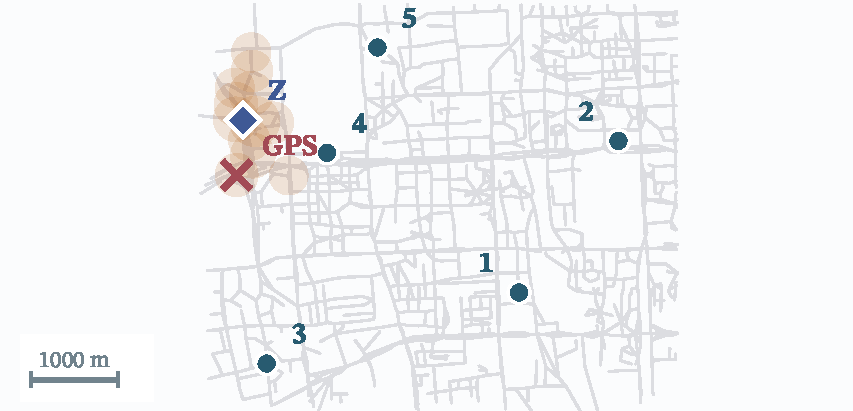
\includegraphics[width=\linewidth]{report_figures/sample_60s.pdf}
{\footnotesize Dấu chéo: GPS; hình thoi: $Z$; điểm 1--5: $Q$.
Màu cam: một phần trọng số $b$, không phải posterior hiệu chuẩn.
© OpenStreetMap contributors.}
\end{minipage}

\subsection{Tại 60 s: lần lượt kích hoạt các cơ chế}
\begin{enumerate}
\item \textbf{Lịch và ngân sách:} đủ 60 s từ lần đọc trước, còn 22/23 đơn vị; dành đủ dự toán $2u$ rồi mới đọc GPS.
\item \textbf{Thử giữ tham chiếu:} khoảng cách GPS tới $Z$ cũ là $3.049{,}59$ m,
$\theta=200$ m, nhiễu $\mathrm{Lap}(800\text{ m})$. Log lưu nhánh thử không đạt, không lưu giá trị nhiễu cụ thể.
\item \textbf{Geo-I/REM:} tạo $Z$ mới. GPS $(39{,}982839;116{,}292335)$;
$Z=(39{,}988552;116{,}293209)$. Chi thêm $2u=0{,}0025/\mathrm m$;
tổng $3u=0{,}00375/\mathrm m$, còn $0{,}025/\mathrm m$.
\item \textbf{Ước lượng và chọn Q:} cập nhật $b$ từ quan sát bảo vệ; chọn năm Q để phủ POI và tiếp tục di chuyển theo đường.
Không dùng GPS thật hoặc nhu cầu riêng để sửa Q.
\item \textbf{Truy hồi chung:} năm Q, L30 mọi loại, gửi ngay. Tổng phản hồi 420 bản ghi;
thiết bị gộp và bỏ trùng còn 252 POI duy nhất qua các loại.
\item \textbf{Nhu cầu local:} dùng GPS và $\psi$ để lọc, sắp xếp trên cùng phản hồi.
Không gửi thêm query khi đổi loại POI, tiêu chí, bán kính hoặc đích riêng.
\end{enumerate}

\par\smallskip
\begin{tabularx}{\linewidth}{@{}P{3.8cm}Y@{}}\toprule
\textbf{Nhu cầu: quán cà phê} & \textbf{Trích kết quả đã lưu, cùng phản hồi tại 60 s}\\\midrule
Gần nhất & Đầu thứ tự: P167, P13, P224, P166, P126.\\
Trong bán kính 1 km & Chỉ còn P167.\\
Ít đi vòng tới đích & Đầu thứ tự: P93, P167, P57, P58, P13.\\\bottomrule
\end{tabularx}
Các danh sách trên trích đầu ra $k=5$ đã lưu, không dựng thêm một danh sách đầy đủ mới.
Ở 600 s, tổng 21/23 tính cả các lần đọc 360/420/480/540 s không hiển thị; mẫu chưa hết cap.

\subsection{Nhánh giữ Z và ranh giới đầu/cuối}
Trong \textbf{phiên 6} của cùng mẫu, tại 60 s có đọc GPS nhưng giữ $Z$: chi $1u$ và cập nhật $b$ từ quan sát giữ.
Đây là nhánh khác với không đọc ở 20 s; không nối phiên 6 vào timeline phiên 1.
Đầu chuyến và các mốc cuối vẫn gửi ngay, không dùng tương lai để biết khi nào cần che phần cuối;
giờ mở/đóng ứng dụng còn có thể lộ.

Mẫu dùng GPS tổng hợp SUMO. Đánh giá utility dùng vị trí thật local tại mỗi mốc 20 s;
đây là oracle đánh giá, không phải phép đo số lần lấy GPS hay năng lượng trên thiết bị thật.

\key{GPS bảo vệ theo lịch; $Z$ và $b$ tạo Q; Q lấy POI; nhu cầu thật chỉ lọc/sắp xếp tại thiết bị.}

\clearpage
\section{Benchmark: cải thiện đã đo và phạm vi kết luận}
\textbf{Đối thủ} nhìn transcript công khai, không nhận GPS thật hay $Z$ của nhánh bảo vệ.
Mỗi phép thử chọn attacker theo task/metric trên tập chọn, không mặc định mọi task đều dùng Shadow kNN.
Hit100 là tỷ lệ suy đúng trong 100 m; MAE là sai số vị trí trung bình; Recall@5 là chất lượng dịch vụ.

\subsection{Utility: L20 và L30 trên cùng Q}
24 nhóm mới trên cùng bản đồ SUMO, 3 lượt nhiễu mỗi nhóm, 8 chuyến/lượt.
Giữ Q, Z, lịch, cap và $k=5$; chỉ đổi độ sâu phản hồi. Macro cho bốn mục đích trọng số đều.
\par\smallskip
\begin{tabularx}{\linewidth}{@{}Yrrr@{}}\toprule
\textbf{Recall@5 $\uparrow$ (\%)} & \textbf{L20} & \textbf{L30} & \textbf{$\Delta$ điểm \%}\\\midrule
\UtilityRows
\bottomrule\end{tabularx}
{\footnotesize Chênh lệch $\Delta$ tính trước làm tròn các cột Recall.}
\key{Macro tăng 2,97 điểm \%; CI 95\% [2,31; 3,65]; ba lượt nhiễu đều tăng.}
Reply JSON $494{,}71\to648{,}58$ MB ($+31{,}10\%$), cùng 90.570 request.
CI bootstrap theo 24 nhóm, không coi tick là subject độc lập. Chưa đo latency, HTTP/TLS hoặc năng lượng.

\textbf{So với báo cáo trước:} L10 đạt Recall 95,44\% cho tìm gần nhất, gộp năm scenario với cache và cap từng chuyến.
Macro L30 92,69\% hiện tại khác purpose, cap, cohort và cách gộp; không lấy chênh hai số làm tăng/giảm trực tiếp.
Replay bốn template L10 không qua gate (86,34\%, byte cao hơn L30 57,52\%); giữ L30.
Replay này dùng lại cohort hiện có, không là xác nhận độc lập mới.

\subsection{Privacy: bằng chứng bổ sung ở các cấu hình riêng}
Đối chứng S4--S6 là GPS thật; đối chứng S9/S10 là Geo-I L20 lịch sử.
\par\smallskip
\begin{tabularx}{\linewidth}{@{}P{2.7cm}P{2.8cm}rrY@{}}\toprule
\textbf{Task} & \textbf{Metric} & \textbf{Đối chứng} & \textbf{Bảo vệ} & \textbf{Cấu hình}\\\midrule
\PrivacyRows
\bottomrule\end{tabularx}

\textbf{S4:} 3 nhóm test/45 cặp; attacker người \textbf{shape/kNN15}, xe \textbf{shape/kNN5} ở raw và \textbf{shape/trees} ở Geo-I.
AUC người từng nhóm còn tới 0,861; AUC dưới 0,5 không chứng minh ẩn danh vì có thể đảo điểm.
Chưa xác nhận linkage cho Epoch8/L30 mới.

\textbf{S5/S6:} pilot Epoch8/L20, 6 nhóm/12 query; \textbf{Candidate Trees} ở raw, \textbf{Motion} ở REM, \textbf{Curve Mean} ở Planar.
Planar cũng đạt 50\%; Recall Planar 97,00\%, REM 94,69\%. Hai task chung quyết định nhị phân, chưa phải dự đoán mọi cạnh/đích.

\textbf{S9/S10:} Endpoint20 gửi ngay, dùng $u=0{,}0025/\mathrm m$ thay $0{,}01/\mathrm m$ của đối chứng L20,
tăng nhiễu ở mọi lần đọc được phép; không phải một phần tư $u$ hiện tại của Epoch8.
28 nhóm đã khảo sát, 112 quan sát/task. Recall $98{,}94\to96{,}64\%$; S10 Hit100 cùng 0\%, CI chênh Hit500 chạm 0.
Attacker chọn riêng theo metric; MAE tăng không chứng minh thắng mọi phép đo.

\key{Đã xác nhận tăng utility có đánh đổi byte. Privacy còn theo từng bank/cấu hình; chưa có một benchmark Epoch8/L30 thống nhất cho S1--S10.}
S1--S3 và đối chứng paper thích nghi giữ ở tài liệu chi tiết; S8 còn mở.
Ưu tiên tiếp theo: xác nhận privacy trên cùng Epoch8/L30, mở rộng linkage và dự đoán tương lai, đo chi phí triển khai.

{\footnotesize\color{gray}\textbf{Nguồn đối chiếu:} \texttt{benchmark\_tables.json}, \texttt{multistep\_sample.json}, \texttt{utility\_sample.json};
báo cáo trước: \texttt{method\_evidence.json} trong thư mục \texttt{2026-09-26\_brief}; mô hình/chứng minh:
\texttt{current\_method.tex}, \texttt{current\_formal\_privacy.tex} trong thư mục \texttt{thesis}.
Hash toàn bộ nguồn: \texttt{report\_sources.json}. Các số đo và đầu ra gốc giữ nguyên.}
\end{document}
